
\subsection*{Projedeki yeri ve araç seçimi}
Projemiz, 5G baz istasyonunun algılama (sensing) için ayırdığı kaynak payının ($\alpha$) haberleşmeye maliyetini ölçmeyi amaçlıyor. ns-3 bu maliyeti \textbf{çok kullanıcılı bir ağda}, yani kullanıcı sayısı arttıkça throughput ve gecikmenin nasıl değiştiğini ölçmek için kullanılacak. ns-3, açık kaynaklı bir ağ simülatörüdür. 5G NR için CTTC'nin geliştirdiği \textbf{5G-LENA} (\texttt{nr} modülü) ns-3'e eklenerek kullanılır. Seçim nedenleri: 5G NR'nin MAC düzeyindeki zamanlayıcılarını (scheduler) içermesi, hazır 5G örnekleri sunması ve akış düzeyinde throughput ile gecikme ölçebilmesi. 5G-LENA her sürüm için belirli bir ns-3 sürümünü önerir; biz \textbf{ns-3.48 + 5G-LENA v5.1} çiftini kullandık.

\subsection*{Kurulum}
\begin{center}\sffamily\small
\begin{tabular}{@{}ll@{}}
\toprule
Ortam & Windows 11 üzerinde WSL2, Ubuntu 24.04.5 LTS \\
Derleyici ve araçlar & g++ 13.3.0, CMake 3.28.3, Ninja \\
Simülatör & ns-3.48 (\texttt{\textasciitilde/ehb415/ns-3-dev}) \\
5G modülü & 5G-LENA v5.1 (\texttt{contrib/nr}) \\
Derleme profili & optimized (\texttt{-d optimized}), 1876 hedef \\
Süre ve disk & yaklaşık 18 dakika (\texttt{-j6}), yaklaşık 0,5 GB \\
\bottomrule
\end{tabular}
\end{center}
Kurulum komutları (Ubuntu terminalinde; ayrıntı: projedeki \texttt{kurulum/04-ns3-5g-lena.md}):
\begin{lstlisting}
sudo apt-get update
sudo apt-get install -y build-essential g++ python3 python3-venv python3-pip cmake \
    ninja-build git ccache pkg-config libc6-dev sqlite3 libsqlite3-dev libeigen3-dev
mkdir -p ~/ehb415 && cd ~/ehb415
git clone --depth 1 --branch ns-3.48 https://gitlab.com/nsnam/ns-3-dev.git
git clone --depth 1 --branch v5.1 https://gitlab.com/cttc-lena/nr.git ns-3-dev/contrib/nr
cd ns-3-dev
./ns3 configure --enable-examples -d optimized -G Ninja
./ns3 build -j6
\end{lstlisting}
5G-LENA klasörünün adı \texttt{nr} olmalı ve \texttt{contrib/} altında durmalı.

\subsection*{Karşılaşılan sorunlar ve çözümleri}
\begingroup\sffamily\small
\begin{xltabular}{\textwidth}{@{}p{4.3cm}X@{}}
\toprule
\textbf{Sorun} & \textbf{Neden ve çözüm} \\
\midrule
\texttt{WSL2 is unable to start since virtualization is not enabled} & WSL kurulduktan sonra gerçek yeniden başlatma yapılmamıştı. Windows'ta Hızlı Başlatma açıkken Kapat--aç yetmiyor. \textbf{Başlat $\rightarrow$ Güç $\rightarrow$ Yeniden başlat} ile çözüldü. \\
Derleme sırasında \texttt{Killed} & Bellek yetmiyor. \texttt{.wslconfig} dosyasında \texttt{memory=10GB} ayarlandı, \texttt{-j6} yerine gerekirse \texttt{-j4} veya \texttt{-j2} kullanılır. \\
PowerShell'den \texttt{wsl -- bash -c '...'} ile karmaşık komutlar bozuluyor & Tırnak ve \texttt{\$}, \texttt{|} gibi karakterler PowerShell ile bash arasında karışıyor. Komutlar bir \texttt{.sh} dosyasına yazılıp \texttt{wsl -- bash dosya.sh} ile çalıştırıldı. \\
Simülasyon çıktısında \texttt{NS\_LOG} mesajları yok & ``optimized'' profilde günlük (log) çıktıları derlemeden çıkarılıyor. Sonuçlar akış izleyicisi (FlowMonitor) ve \texttt{trace} geri çağırmalarından okunuyor. Günlük gerekirse \texttt{-d debug} ile yeniden yapılandırılır. \\
Başka ns-3 sürümüyle derleme denemesi & 5G-LENA v5.1, ns-3.48 için tasarlandı; ns-3.49 gibi sürümlerle denenmemeli. \\
\bottomrule
\end{xltabular}
\endgroup

\subsection*{Örnek çalıştırma}
\subsubsection*{5G-LENA'nın hazır örneği: \texttt{cttc-nr-demo}}
Kurulumun doğru olduğunu görmek için 5G-LENA örneğini 2 kullanıcı ve 1 saniye simülasyonla çalıştırdım.
\begin{figure}[h!]
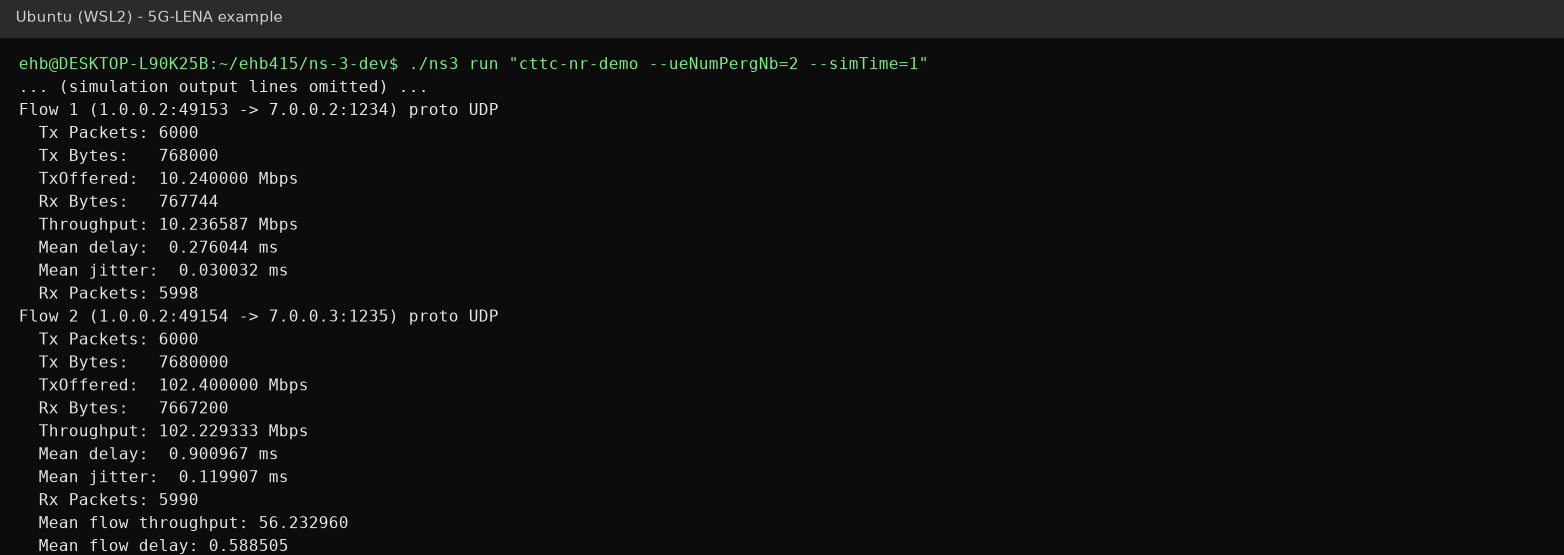
\includegraphics[width=\textwidth]{img/ns3_rapor_demo.png}
\caption{\texttt{cttc-nr-demo} çıktısının akış sonuçları (WSL2 Ubuntu terminali).}
\end{figure}

\begin{center}\sffamily\small
\begin{tabular}{@{}lrrrr@{}}
\toprule
 & Gönderilen & Alınan & Gecikme & Paket kaybı \\
\midrule
Akış 1 & 10,24 Mbps & 10,24 Mbps & 0,28 ms & \%0,03 \\
Akış 2 & 102,40 Mbps & 102,23 Mbps & 0,90 ms & \%0,17 \\
Ortalama (\texttt{Mean flow}) & & 56,23 Mbps & 0,59 ms & \\
\bottomrule
\end{tabular}
\end{center}
Alınan veri gönderilene çok yakın ve gecikme 1\,ms altında. Yük kapasitenin altında olduğu için bu beklenen bir sonuç.

\subsubsection*{Kendi yazdığım basit uygulama}
ns-3'ün nasıl çalıştığını anlamak için iki bilgisayar ve aralarında bir kablodan oluşan program yazdım (\texttt{scratch/benim\_ilk.cc}). Kablo 5\,Mbps hızında ve 500\,ms gecikmeli; istemci t\,=\,2\,s'de 1024 baytlık tek paket yolluyor, sunucu cevap veriyor.
\begin{figure}[h!]
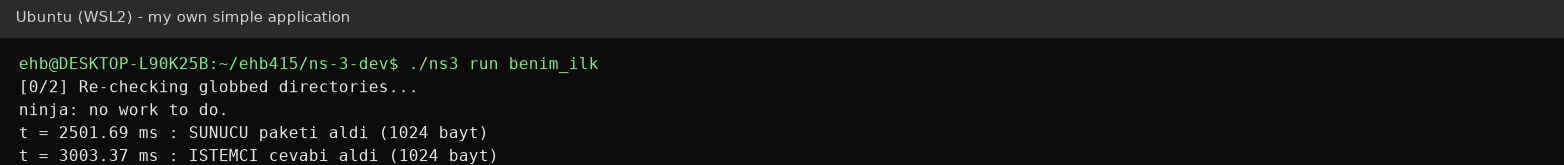
\includegraphics[width=\textwidth]{img/ns3_rapor_ilk.png}
\caption{\texttt{./ns3 run benim\_ilk} çıktısı.}
\end{figure}
Elle hesap: paket başlıklarıyla 1054 bayt, $1054\times 8/5\,\text{Mbps}=1{,}69$\,ms, artı 500\,ms kablo gecikmesi $=501{,}69$\,ms. Sunucu paketi $2000+501{,}69=2501{,}69$\,ms'de aldı, cevap aynı yoldan dönünce istemci $3003{,}37$\,ms'de aldı. Simülasyon çıktısı elle hesapla birebir tuttu.

\subsection*{Değerlendirme ve sonraki adımlar}
ns-3.48 ve 5G-LENA v5.1 kuruldu, derlendi ve hem hazır 5G örneği hem kendi programım doğru sonuç üretti. Sınırlamalar: 5G-LENA'da hazır bir sensing modeli yok, bu yüzden ns-3 yalnızca haberleşme tarafının maliyetini ölçecek; sensing yükünü simülasyonda temsil etme yolu henüz seçilmedi. Sonraki adımlar:
\begin{itemize}
\item Kullanıcı sayısını (1, 2, 5, 10, 20) değiştirip toplam throughput ve gecikmeyi ölçmek.
\item 5G-LENA'daki zamanlayıcıları (\texttt{nr-mac-scheduler-*}) incelemek; varsayılan olan \texttt{NrMacSchedulerTdmaRR}'dir.
\item Bandı daraltarak sensing yükünü taklit eden deney ve bunun alternatifi olan ``sensing'i ayrı trafik akışı olarak ekleme'' yollarını karşılaştırmak.
\end{itemize}
